% set document class as 'report'
% set default font size as '12pt'
\documentclass[12pt]{report}

\usepackage[utf8]{inputenc}

% ====== for reference clickable ======
\usepackage{hyperref}
% ====== for graphics ======
\usepackage{graphicx} % includegraphic 
\usepackage{placeins} % FloatBarrier 
% ====== set Font Family ======
\usepackage{mathptmx} % Font: Times
% ====== set margin here ======
\usepackage{geometry}
\geometry{
 a4paper, % set A4 paper
 right=1in, % set margin 1 inch
 bottom=1in, % set margin 1 inch
 top=1in, % set margin 1 inch
 left=3cm % set margin 1.5 inch
 }
% ====== for styling Table of Content =====
\usepackage{tocloft}
% ====== for styling 'chapter' and 'section' ...
\usepackage{titlesec}

% Chapter
\titleformat
{\chapter} % command
[display] % shape
{\bfseries\large\center} % format
{CHAPTER \thechapter} % label
{0.6em} % sep
{} % before-code
[] % after-code
% remove space above and set below 28pt space chapter
\titlespacing*{\chapter}{0pt}{-35pt}{28pt}

% Section (Heading, Level 2)
\titleformat
{\section} % command
[hang] % shape
{\bfseries} % format
{\thesection} % label
{0em} % sep
{ } % before-code
[] % after-code
% add 1.5 line space above section and remove line space after it
\titlespacing*{\section}{0pt}{1.6em}{0pt}

% subSection (Heading, Level 3)
\titleformat
{\subsection} % command
[hang] % shape
{\bfseries \itshape} % format
{\thesubsection} % label
{0em} % sep
{ } % before-code
[] % after-code
% add 0 line space above section and remove line space after it
\titlespacing*{\subsection}{0pt}{0em}{0pt}

% subsubSection (Heading, Level 4)
\titleformat
{\subsubsection} % command
[runin] % shape
{\bfseries} % format
{\thesubsubsection} % label
{0em} % sep
{ } % before-code
[] % after-code
% 0.5inch indent, 0 line space above, 1 space after header
\titlespacing*{\subsubsection}{0.5in}{0em}{1ex}

% ====== Indent ======
% By default, the first paragraph is not indent - we need this package for indentation
\usepackage{indentfirst}
% ====== list + enum ======
\usepackage{enumitem}
% Set indent lenght for itemize and enumerate
\setlist[itemize]{left=0.5in}
\setlist[enumerate]{left=0.5in}
% Remove separation between item
\setlist{nosep}
% ====== caption styling ======
\usepackage{caption}
\DeclareCaptionFormat{aitformat}{\textbf{#1} #2 \textit{#3}}
% justification = RaggedRight : Caption start on the left
% singlelinecheck = false     : Force caption to start on the left
% labelsep = newline          : separate Table 1.1 and label
\captionsetup{format = aitformat,
              justification = RaggedRight,
              singlelinecheck = false,
              labelsep = newline}
              
% ====== References ======
\usepackage[notocbib]{apacite}

% ====== Document begins here ======
\begin{document}
    % Set counter depth up to subsubsection (heading, level 4)
    \setcounter{secnumdepth}{3}
    
    % ====== include other section ======
    \begin{titlepage}
%   everything on center
  \begin{center}
   
  \textbf{\large{
  MITOCHONDRIAL DNA CHARACTERIZATION OF INDIGENOUS STRAINS OF COMMON CARP (Cyprinus carpio)
  }}

  \vspace{3em} % (3 blank lines)
  
  by
  
  \vspace{3em} % (3 blank lines)
  
  Write your full name here.
  
  \vspace{4em} % (4 blank lines)

  A Thesis Submitted in Partial Fulfillment of the Requirements for the Degree of Master of Science in Aquaculture and Aquatic Resources Management

  \vspace{4em} % (4 blank lines)

\begin{center}
  \begin{tabular}{ rl }
Examination Committee: & Name of Chairperson (Chairperson) \\
                       & Committee Member \\ 
                       & Committee Member \\\\
                       
% UNCOMMENT THE LINES BELOW IF YOU HAVE THE EXTERNAL EXAMINER.
% External Examiner: & Prof. YOUR EXTERNAL EXAMINER  \\
%                   & Dept. of Electrical and Computer Engineering \\ 
%                   & McGill University, Canada \\ \\
\\ \\ \\
Nationality:     & Thai \\
Previous Degree: & Bachelor of Engineering in Computer Engineering \\
                 & Kasetsart University \\
                 & Thailand \\
\\
% *  For Self-Support – delete the line Scholarship Donor
Scholarship Donor: & Government of Switzerland*
  \end{tabular}
\end{center}

\vspace{4em}

Asian Institute of Technology \\
School of Engineering and Technology \\
Thailand \\ 
% (month and year of graduation)          
April 2002


  \end{center}
\end{titlepage}

    
    % Show page numbering as 'roman'
    \pagenumbering{roman}
    % Start page counter as 2
    \setcounter{page}{2}
    
    % add to Table of content
\addcontentsline{toc}{part}{ACKNOWLEDGMENTS}

% set 0 indentation
\setlength{\parindent}{0pt}
% set paragraph space = 1 space
\setlength{\parskip}{1em}
% set line space = 1
\setlength{\baselineskip}{1.2em} % this is the default value for line space = 1

\begin{center}
  \fontsize{14}{17}\selectfont{\textbf{
    ACKNOWLEDGMENTS
  }} \\
\end{center}
\vspace{36pt} 

Lorem ipsum dolor sit amet, consectetur adipiscing elit, sed do eiusmod tempor incididunt ut labore et dolore magna aliqua. Aliquam malesuada bibendum arcu vitae elementum. Aliquet enim tortor at auctor. Sodales ut eu sem integer vitae justo. Tellus pellentesque eu tincidunt tortor aliquam nulla facilisi. Ut lectus arcu bibendum at varius vel pharetra. Integer vitae justo eget magna. Mollis nunc sed id semper risus. Donec ac odio tempor orci dapibus ultrices in iaculis. Non arcu risus quis varius quam quisque id diam vel. Felis donec et odio pellentesque diam volutpat commodo sed egestas. Dignissim diam quis enim lobortis scelerisque. Placerat vestibulum lectus mauris ultrices eros in cursus.

Ut venenatis tellus in metus vulputate eu scelerisque felis. Blandit volutpat maecenas volutpat blandit aliquam etiam erat velit. Ac felis donec et odio pellentesque diam volutpat commodo sed. Dignissim convallis aenean et tortor at risus viverra adipiscing at. Donec pretium vulputate sapien nec. Nisi porta lorem mollis aliquam. Sed nisi lacus sed viverra. Metus vulputate eu scelerisque felis imperdiet proin fermentum leo vel. Convallis convallis tellus id interdum velit laoreet id donec ultrices. Volutpat diam ut venenatis tellus in metus. Magna fringilla urna porttitor rhoncus dolor purus non enim. Eget mi proin sed libero enim sed faucibus turpis in. Bibendum ut tristique et egestas quis ipsum suspendisse. Tellus integer feugiat scelerisque varius morbi. Aliquet eget sit amet tellus. Massa tincidunt dui ut ornare lectus sit. Nunc scelerisque viverra mauris in aliquam sem fringilla. Cum sociis natoque penatibus et magnis dis parturient montes nascetur. Et egestas quis ipsum suspendisse ultrices. Mauris vitae ultricies leo integer malesuada nunc vel risus.
    % add to Table of content
\addcontentsline{toc}{part}{ABSTRACT}

% set 0 indentation
\setlength{\parindent}{0pt}
% set paragraph space = 1 space
\setlength{\parskip}{1em}
% set line space = 1.5
\setlength{\baselineskip}{1.5em}

\begin{center}
  \fontsize{14}{17}\selectfont{\textbf{
    ABSTRACT
  }}
\end{center}
\vspace{2em}

Lorem ipsum dolor sit amet, consectetur adipiscing elit, sed do eiusmod tempor incididunt ut labore et dolore magna aliqua. Aliquam malesuada bibendum arcu vitae elementum. Aliquet enim tortor at auctor. Sodales ut eu sem integer vitae justo. Tellus pellentesque eu tincidunt tortor aliquam nulla facilisi. Ut lectus arcu bibendum at varius vel pharetra. Integer vitae justo eget magna. Mollis nunc sed id semper risus. Donec ac odio tempor orci dapibus ultrices in iaculis. Non arcu risus quis varius quam quisque id diam vel. Felis donec et odio pellentesque diam volutpat commodo sed egestas. Dignissim diam quis enim lobortis scelerisque. Placerat vestibulum lectus mauris ultrices eros in cursus.

Ut venenatis tellus in metus vulputate eu scelerisque felis. Blandit volutpat maecenas volutpat blandit aliquam etiam erat velit. Ac felis donec et odio pellentesque diam volutpat commodo sed. Dignissim convallis aenean et tortor at risus viverra adipiscing at. Donec pretium vulputate sapien nec. Nisi porta lorem mollis aliquam. Sed nisi lacus sed viverra. Metus vulputate eu scelerisque felis imperdiet proin fermentum leo vel. Convallis convallis tellus id interdum velit laoreet id donec ultrices. Volutpat diam ut venenatis tellus in metus. Magna fringilla urna porttitor rhoncus dolor purus non enim. Eget mi proin sed libero enim sed faucibus turpis in. Bibendum ut tristique et egestas quis ipsum suspendisse. Tellus integer feugiat scelerisque varius morbi. Aliquet eget sit amet tellus. Massa tincidunt dui ut ornare lectus sit. Nunc scelerisque viverra mauris in aliquam sem fringilla. Cum sociis natoque penatibus et magnis dis parturient montes nascetur. Et egestas quis ipsum suspendisse ultrices. Mauris vitae ultricies leo integer malesuada nunc vel risus.


\textbf{Keywords:} keyword1, keyword2. 
    % Rename table of content to CONTENTS
\renewcommand\contentsname{\begin{center}
  \fontsize{14}{17}\selectfont{\bf{CONTENTS}}
\end{center}}
% set space above title
\renewcommand{\cftbeforetoctitleskip}{-35pt}
% set space below title
\renewcommand{\cftaftertoctitleskip}{0em}
% after title, skip 3 spaces and write 'page' on the right
\renewcommand{\cftaftertoctitle}{%
  \vspace{3em}
  \hfill{\textbf{Page}}
}
% Remove . from table of content
\renewcommand{\cftdot}{}

% styling part:
\renewcommand{\cftpartfont}{\fontsize{12}{14}\selectfont\bf} % set font bold for page name
\renewcommand{\cftpartpagefont}{\fontsize{12}{14}\selectfont\bf} % set font size and bold for page number
\setlength{\cftbeforepartskip}{0pt} % set line space

% styling chapter:
\renewcommand{\cftchapfont}{\bf{CHAPTER} \fontsize{12}{14}\selectfont\bf} % set font size bold, leading with 'CHAPTER'
\renewcommand{\cftchappagefont}{\fontsize{12}{14}\selectfont\bf} % set font size and bold for page number
\setlength{\cftbeforechapskip}{0pt} % set line space
\setlength{\cftsecindent}{4.5em}
\setlength{\cftsubsecindent}{7em}

% set dept of contents
\setcounter{tocdepth}{2}

% Print content
\tableofcontents
    \addcontentsline{toc}{part}{LIST OF TABLES}

% Rename List of Tables to CONTENTS
\renewcommand\listtablename{\begin{center}
  \fontsize{14}{17}\selectfont{LIST OF TABLES}
\end{center}}
% set space above title
\renewcommand{\cftbeforelottitleskip}{-25pt}
% set space below title
\renewcommand{\cftafterlottitleskip}{0em}
% after title, skip 3 spaces and write 'page' on the right
\renewcommand{\cftafterlottitle}{%
  \vspace{3em}
  \textbf{Tables}\hfill{\textbf{Page}}
}

% remove indent
\renewcommand{\cfttabindent}{0pt}
% add 'Table' before numbering
\renewcommand{\cfttabpresnum}{Table~}
% indent the table caption
\renewcommand{\cfttabnumwidth}{4.5em}

\begingroup
    \renewcommand*{\addvspace}[1]{}
    \listoftables
\endgroup
    \addcontentsline{toc}{part}{LIST OF FIGURES}

% Rename List of Tables to CONTENTS
\renewcommand\listfigurename{\begin{center}
  \fontsize{14}{17}\selectfont{LIST OF FIGURES}
\end{center}}
% set space above title
\renewcommand{\cftbeforeloftitleskip}{-25pt}
% set space below title
\renewcommand{\cftafterloftitleskip}{0em}
% after title, skip 3 spaces and write 'page' on the right
\renewcommand{\cftafterloftitle}{%
  \vspace{3em}
  \textbf{Figures}\hfill{\textbf{Page}}
}

% remove indent
\renewcommand{\cftfigindent}{0pt}
% add 'Table' before numbering
\renewcommand{\cftfigpresnum}{Figure~}
% indent the table caption
\renewcommand{\cftfignumwidth}{4.5em}

\begingroup
    \renewcommand*{\addvspace}[1]{}
    \listoffigures
\endgroup
    
    % Start page counter as 1
    \setcounter{page}{1}
    % Show page numbering as 'arabic'
    \pagenumbering{arabic}
    % set 0.5 inch indentation
\setlength{\parindent}{0.5in} 
% set paragraph space = 0 space
\setlength{\parskip}{0mm}
% set line space 1.5
\setlength{\baselineskip}{1.6em}

\chapter{INTRODUCTION} 

\section{Background of the Study}
Start your paragraph here; justified, 0.5” indentation. Maintain a 1.5 line spacing throughout. This section should consist of 2 pages maximum excluding figures and tables. This is NOT a Literature Review section.

Each paragraph should have at least 4 sentences. Paragraphs of more than 6 sentences should be split into two paragraphs. Follow the appropriate structure of writing a clear paragraph.  Consult your adviser about the subsections. Maintain one space between the last line of this section and the next subsection.

\section{Statement of the Problem}
Write approximately three paragraphs only. Each paragraph should have at least 4 sentences. Paragraphs of more than 6 sentences should be split into two paragraphs. Follow the appropriate structure of writing a clear paragraph.

\section{Research Questions- Discuss with your adviser.}
Introduce your research questions in one sentence followed by a bulleted list, left-aligned.

\begin{enumerate}
    \item Follow a 0.5” Tab setting
    \item
    \item
\end{enumerate}

\section{Objectives of the Study}
Introduce your main objective first in one sentence, followed by a bulleted list of specific objectives, left aligned.
\begin{itemize}
    \item Follow a 0.5” Tab setting
    \item
    \item
\end{itemize}

\section{Write the next section here.}
Start your paragraph here. 

\section{Organization of the Thesis}
Start your paragraph here. 


\begin{table}[ht]
  \caption[Random Table]{Random Table}
  \begin{center}
    \begin{tabular}{cccc}
      \hline \textbf{v1} & \textbf{v2} & \textbf{v3} & \textbf{Overall} \\ \hline
        78.67\% & 87.33\% & 94.92\% & 85.64\% \\ \hline
    \end{tabular}
  \end{center}
  \label{tab:random_table}
\end{table} 

\begin{table}[ht]
  \caption[Random Table 2]{Random Table 2}
  \begin{center}
    \begin{tabular}{cccc}
      \hline \textbf{v1} & \textbf{v2} & \textbf{v3} & \textbf{Overall} \\ \hline
        78.67\% & 87.33\% & 94.92\% & 85.64\% \\ \hline
    \end{tabular}
  \end{center}
  \label{tab:random_table_2}
\end{table} 

\begin{figure}[ht]
  \centering
  \caption[Random Figure]{Random Figure}
  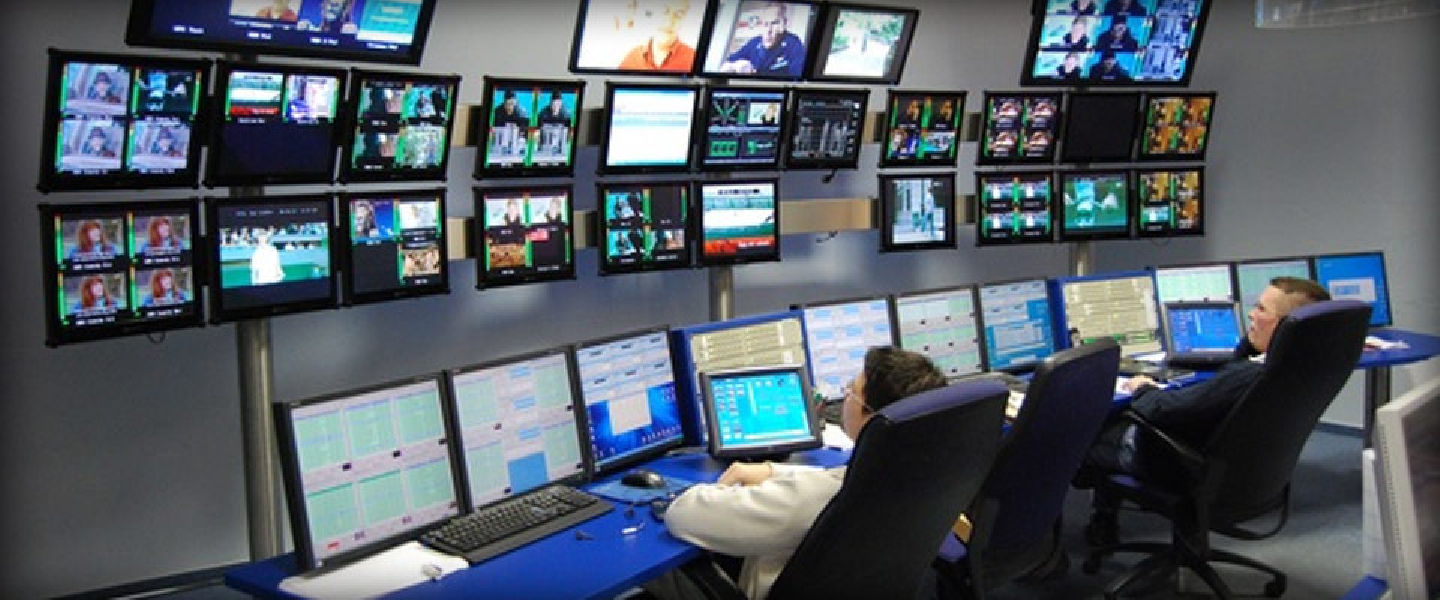
\includegraphics[width=0.75\textwidth]{figures/monitoring.pdf}
  \label{fig:random_figure}
\end{figure}
    % % set 0.5 inch indentation
\setlength{\parindent}{0.5in} 
% set paragraph space = 0 space
\setlength{\parskip}{0mm}
% set line space 1.5
\setlength{\baselineskip}{1.6em}

\chapter{TITLE}
Write your introductory paragraph/s here (except for Chapter 1). Limit this section to two paragraphs. Follow the appropriate structure of writing paragraphs. Paragraphs should have at least four sentences. Paragraphs with more than 6 sentences must be split into two paragraphs.

\section{Heading, Level 2}
Start your paragraph here.
\section{Heading, Level 2}
Start your paragraph here.
\subsection{Heading, Level 3}
Start your paragraph here.
\subsection{Heading, Level 3}
Start your paragraph here.
\section{Heading, Level 2}
Start your paragraph here.
\subsection{Heading, Level 3}
Start your paragraph here.
\subsection{Heading, Level 3}
Start your paragraph here.
\subsubsection{Heading, Level 4}
Start on the same line here and continue as a regular paragraph.
\subsubsection{Heading, Level 4}
Start on the same line here and continue as a regular paragraph.
\section{Heading, Level 2}
Start your paragraph here.
    % set 0.5 inch indentation
\setlength{\parindent}{0.5in} 
% set paragraph space = 0 space
\setlength{\parskip}{0mm}
% set line space 1.5
\setlength{\baselineskip}{1.6em}

\chapter{LITERATURE REVIEW}
\label{ch:literature-review}
Write your introductory paragraph/s here (except for Chapter 1). Limit this section to two paragraphs. Follow the appropriate structure of writing paragraphs. Paragraphs should have at least four sentences. Paragraphs with more than 6 sentences must be split into two paragraphs.

\section{Section Name in Literature Review}
\label{section-name-in-literature-review}

\shortciteA{yamato92hmm} apply the background subtraction 
technique to extract blobs or human from a scene by the 
following conditions:
\[
\begin{array}{lc}
  {\rm if} & \left|{I_a (x,y) - I_b (x,y)}\right|< T,\;I_e (x,y) = 0 \\ 
  {\rm else} & I_e (x,y) = I_a (x,y), 
\end{array}
\]
where $I_e (x,y)$ is a human extracted image, $I_a (x,y)$ is an
original image, $I_b (x,y)$ is a background image, and $T$ is a
threshold. Figure~\ref{fig:mesh-feature} shows something. Some work also uses 
mesh features~\shortcite{yamato92hmm}.

% THE REASON ~ IS USED HERE BECAUSE WE TELL LATEX THAT THESE TWO WORDS SHOULD 
% GO TOGETHER IN THE SAME LINE.

\begin{figure}[h]
  \centering
  \caption[Mesh feature calculation]{Mesh feature calculation. Reprinted from the work of Yamato et al.\ (1992).}
  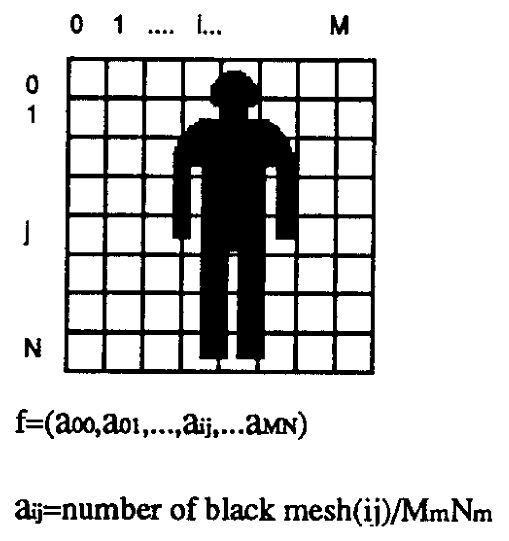
\includegraphics[width=2in]{figures/mesh-feature.jpg}  
  \label{fig:mesh-feature}
\end{figure}

\begin{table}[ht]
  \caption[Random Table 3]{Random Table 3}
  \begin{center}
    \begin{tabular}{cccc}
      \hline \textbf{v1} & \textbf{v2} & \textbf{v3} & \textbf{Overall} \\ \hline
        78.67\% & 87.33\% & 94.92\% & 85.64\% \\ \hline
    \end{tabular}
  \end{center}
  \label{tab:random_table_3}
\end{table} 

\section{Chapter Summary}
All chapters except Chapter 1 must include an introductory paragraph/s and a chapter summary.

\FloatBarrier
    % set 0.5 inch indentation
\setlength{\parindent}{0.5in} 
% set paragraph space = 0 space
\setlength{\parskip}{0mm}
% set line space 1.5
\setlength{\baselineskip}{1.6em}

\chapter{METHODOLOGY}
\label{ch:methodology}
Write your introductory paragraph/s here (except for Chapter 1). Limit this section to two paragraphs. Follow the appropriate structure of writing paragraphs. Paragraphs should have at least four sentences. Paragraphs with more than 6 sentences must be split into two paragraphs.

\section{Your section}
Lorem ipsum dolor sit amet, consectetur adipiscing elit, sed do eiusmod tempor incididunt ut labore et dolore magna aliqua. Aliquam malesuada bibendum arcu vitae elementum. Aliquet enim tortor at auctor. Sodales ut eu sem integer vitae justo. Tellus pellentesque eu tincidunt tortor aliquam nulla facilisi. Ut lectus arcu bibendum at varius vel pharetra. Integer vitae justo eget magna. Mollis nunc sed id semper risus. Donec ac odio tempor orci dapibus ultrices in iaculis. Non arcu risus quis varius quam quisque id diam vel. Felis donec et odio pellentesque diam volutpat commodo sed egestas. Dignissim diam quis enim lobortis scelerisque. Placerat vestibulum lectus mauris ultrices eros in cursus.

Ut venenatis tellus in metus vulputate eu scelerisque felis. Blandit volutpat maecenas volutpat blandit aliquam etiam erat velit. Ac felis donec et odio pellentesque diam volutpat commodo sed. Dignissim convallis aenean et tortor at risus viverra adipiscing at. Donec pretium vulputate sapien nec. Nisi porta lorem mollis aliquam. Sed nisi lacus sed viverra. Metus vulputate eu scelerisque felis imperdiet proin fermentum leo vel. Convallis convallis tellus id interdum velit laoreet id donec ultrices. Volutpat diam ut venenatis tellus in metus. Magna fringilla urna porttitor rhoncus dolor purus non enim. Eget mi proin sed libero enim sed faucibus turpis in. Bibendum ut tristique et egestas quis ipsum suspendisse. Tellus integer feugiat scelerisque varius morbi. Aliquet eget sit amet tellus. Massa tincidunt dui ut ornare lectus sit. Nunc scelerisque viverra mauris in aliquam sem fringilla. Cum sociis natoque penatibus et magnis dis parturient montes nascetur. Et egestas quis ipsum suspendisse ultrices. Mauris vitae ultricies leo integer malesuada nunc vel risus.

\section{Chapter Summary}
All chapters except Chapter 1 must include an introductory paragraph/s and a chapter summary.

\FloatBarrier
    % set 0.5 inch indentation
\setlength{\parindent}{0.5in} 
% set paragraph space = 0 space
\setlength{\parskip}{0mm}
% set line space 1.5
\setlength{\baselineskip}{1.6em}

\chapter{EXPERIMENTAL RESULTS}
Write your introductory paragraph/s here (except for Chapter 1). Limit this section to two paragraphs. Follow the appropriate structure of writing paragraphs. Paragraphs should have at least four sentences. Paragraphs with more than 6 sentences must be split into two paragraphs.

\section{Your section}
Lorem ipsum dolor sit amet, consectetur adipiscing elit, sed do eiusmod tempor incididunt ut labore et dolore magna aliqua. Aliquam malesuada bibendum arcu vitae elementum. Aliquet enim tortor at auctor. Sodales ut eu sem integer vitae justo. Tellus pellentesque eu tincidunt tortor aliquam nulla facilisi. Ut lectus arcu bibendum at varius vel pharetra. Integer vitae justo eget magna. Mollis nunc sed id semper risus. Donec ac odio tempor orci dapibus ultrices in iaculis. Non arcu risus quis varius quam quisque id diam vel. Felis donec et odio pellentesque diam volutpat commodo sed egestas. Dignissim diam quis enim lobortis scelerisque. Placerat vestibulum lectus mauris ultrices eros in cursus.

Ut venenatis tellus in metus vulputate eu scelerisque felis. Blandit volutpat maecenas volutpat blandit aliquam etiam erat velit. Ac felis donec et odio pellentesque diam volutpat commodo sed. Dignissim convallis aenean et tortor at risus viverra adipiscing at. Donec pretium vulputate sapien nec. Nisi porta lorem mollis aliquam. Sed nisi lacus sed viverra. Metus vulputate eu scelerisque felis imperdiet proin fermentum leo vel. Convallis convallis tellus id interdum velit laoreet id donec ultrices. Volutpat diam ut venenatis tellus in metus. Magna fringilla urna porttitor rhoncus dolor purus non enim. Eget mi proin sed libero enim sed faucibus turpis in. Bibendum ut tristique et egestas quis ipsum suspendisse. Tellus integer feugiat scelerisque varius morbi. Aliquet eget sit amet tellus. Massa tincidunt dui ut ornare lectus sit. Nunc scelerisque viverra mauris in aliquam sem fringilla. Cum sociis natoque penatibus et magnis dis parturient montes nascetur. Et egestas quis ipsum suspendisse ultrices. Mauris vitae ultricies leo integer malesuada nunc vel risus.

\section{Chapter Summary}
All chapters except Chapter 1 must include an introductory paragraph/s and a chapter summary.

\FloatBarrier
    % set 0.5 inch indentation
\setlength{\parindent}{0.5in} 
% set paragraph space = 0 space
\setlength{\parskip}{0mm}
% set line space 1.5
\setlength{\baselineskip}{1.6em}

\chapter{CONCLUSION}
Write your introductory paragraph/s here (except for Chapter 1). Limit this section to two paragraphs. Follow the appropriate structure of writing paragraphs. Paragraphs should have at least four sentences. Paragraphs with more than 6 sentences must be split into two paragraphs.

\section{Your section}
Lorem ipsum dolor sit amet, consectetur adipiscing elit, sed do eiusmod tempor incididunt ut labore et dolore magna aliqua. Aliquam malesuada bibendum arcu vitae elementum. Aliquet enim tortor at auctor. Sodales ut eu sem integer vitae justo. Tellus pellentesque eu tincidunt tortor aliquam nulla facilisi. Ut lectus arcu bibendum at varius vel pharetra. Integer vitae justo eget magna. Mollis nunc sed id semper risus. Donec ac odio tempor orci dapibus ultrices in iaculis. Non arcu risus quis varius quam quisque id diam vel. Felis donec et odio pellentesque diam volutpat commodo sed egestas. Dignissim diam quis enim lobortis scelerisque. Placerat vestibulum lectus mauris ultrices eros in cursus.

Ut venenatis tellus in metus vulputate eu scelerisque felis. Blandit volutpat maecenas volutpat blandit aliquam etiam erat velit. Ac felis donec et odio pellentesque diam volutpat commodo sed. Dignissim convallis aenean et tortor at risus viverra adipiscing at. Donec pretium vulputate sapien nec. Nisi porta lorem mollis aliquam. Sed nisi lacus sed viverra. Metus vulputate eu scelerisque felis imperdiet proin fermentum leo vel. Convallis convallis tellus id interdum velit laoreet id donec ultrices. Volutpat diam ut venenatis tellus in metus. Magna fringilla urna porttitor rhoncus dolor purus non enim. Eget mi proin sed libero enim sed faucibus turpis in. Bibendum ut tristique et egestas quis ipsum suspendisse. Tellus integer feugiat scelerisque varius morbi. Aliquet eget sit amet tellus. Massa tincidunt dui ut ornare lectus sit. Nunc scelerisque viverra mauris in aliquam sem fringilla. Cum sociis natoque penatibus et magnis dis parturient montes nascetur. Et egestas quis ipsum suspendisse ultrices. Mauris vitae ultricies leo integer malesuada nunc vel risus.

\section{Chapter Summary}
All chapters except Chapter 1 must include an introductory paragraph/s and a chapter summary.

\FloatBarrier
    
    % ====== Reference part ======
    % https://ctan.math.illinois.edu/macros/latex/contrib/apacite/apacite.pdf
    \addcontentsline{toc}{part}{REFERENCES}
    % change page title
    \renewcommand\bibname{REFERENCES}
    \bibliographystyle{apacite}
    \bibliography{references}
    % ====== ======
    \addtocontents{toc}{\bf{APPENDICES}}
    % add to Table of content
\addcontentsline{toc}{section}{\bf{APPENDIX A: SURVEY QUESTIONNAIRE}}

% set 0 indentation
\setlength{\parindent}{0pt}
% set paragraph space = 1 space
\setlength{\parskip}{1em}
% set line space = 1.5
\setlength{\baselineskip}{1.5em}

\begin{center}
  \fontsize{14}{17}\selectfont{\textbf{
    APPENDIX A
  }}\\
  \fontsize{14}{25}\selectfont{\textbf{
    SURVEY QUESTIONNAIRE
  }}
\end{center}
% \vspace{0em}

Different materials are presented in the APPENDICES. Label the materials in the order that they are mentioned in the text or section (e.g., “see Appendix A for the questions”). Large or oversized tables or figures that support, but are not important in the text, are included in the appendices in a portrait or landscape orientation.


    % add to Table of content
\addcontentsline{toc}{section}{\bf{APPENDIX B: TITLE}}

% set 0 indentation
\setlength{\parindent}{0pt}
% set paragraph space = 1 space
\setlength{\parskip}{1em}
% set line space = 1.5
\setlength{\baselineskip}{1.5em}

\renewcommand{\thefigure}{B\arabic{figure}}
\renewcommand{\thetable}{B\arabic{table}}

\begin{center}
  \fontsize{14}{17}\selectfont{\textbf{
    APPENDIX B
  }}\\
  \fontsize{14}{25}\selectfont{\textbf{
    TITLE
  }}
\end{center}
% \vspace{1em}

Multiple texts, tables and/or figures can be combined in one appendix.  They should be referred to in a section or parts of your thesis. Number and title the materials in the order they are mentioned in the sections. Add a short description of Appendix A.  Do the same for other appendices with multiple materials.

\begin{figure}[ht]
  \centering
  \caption[CCTV monitoring room in Appendix B.]{CCTV monitoring room. Reprinted from the Twenty First Security Web site (\url{http://www.twentyfirstsecurity.com.au/}).}
  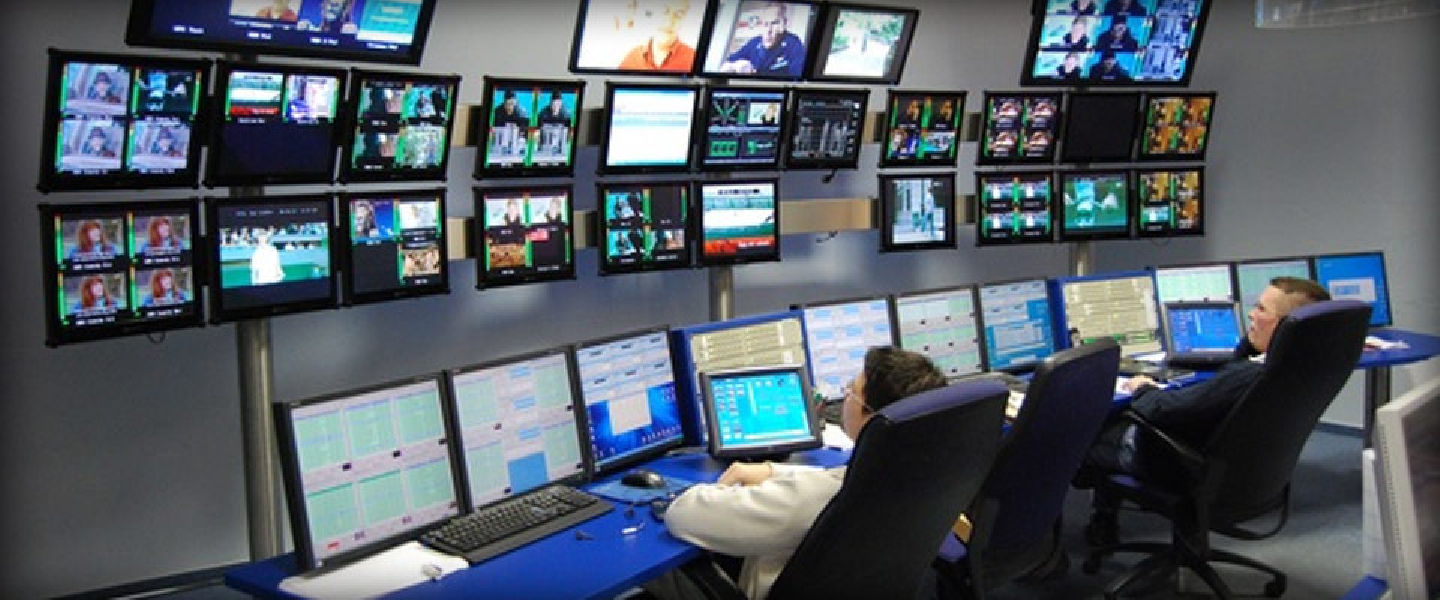
\includegraphics[width=5in]{figures/monitoring}
  \label{fig:monitoring-test}
\end{figure}

\begin{table}[ht]
  \caption[Random Table B]{Random Table B}
  \begin{center}
    \begin{tabular}{cccc}
      \hline \textbf{v1} & \textbf{v2} & \textbf{v3} & \textbf{Overall} \\ \hline
        78.67\% & 87.33\% & 94.92\% & 85.64\% \\ \hline
    \end{tabular}
  \end{center}
  \label{tab:random_table_B}
\end{table} 
    
\end{document}


